\documentclass{article}
\usepackage[utf8]{inputenc}
\usepackage{graphicx}
\usepackage{hyperref}
\usepackage[export]{adjustbox}
\usepackage{wrapfig}
\usepackage{subcaption}
\usepackage{float}
\usepackage{amsmath}
\usepackage{dirtytalk}

\begin{document}


\begin{titlepage}
   \begin{center}
       \vspace*{0.5cm}

       \textbf{New York City Housing Market}

       \vspace{0.5cm}
        Predicting Home Prices

       \vspace{0.5cm}

       \textbf{Pizon Shetu}

       \vspace{0.5cm}

       September, 2021
   \end{center}

\tableofcontents
\clearpage
\section{Problem}
    New York City(NYC) is one of the largest financial central hub on Earth, it has the 44$^{th}$ largest population of all cities in the world which makes it a prime area for growing real-estate investments. The Housing Market has been booming since the great recession of 2008, as prices keep skyrocketing our client Capital Fortune who are a mid-west real-estate investment trust are seeking an opportunity to capitalize on this growth. They have multiple properties set to be built in the 5 boroughs of New York City by 2025. They are seeking our help with identifying key insights and intrinsic value behind the homes in the 5 boroughs.  \\
    \\
    Capital Fortune is naive to the local market conditions of New York City and are concerned on the pricing of their homes on release to the market, they are afraid if they have a steep asking price they will be left waiting and buyers will flock to older and more competitive homes and lose time and money on their investment. They also do not want to price too low as this will result in not maximizing net-profits. They are also interested in different home structures and which yield the greatest net-profits \\
    \\
    As a native New York resident I am decently knowledgeable on our local housing markets but I need to do some analysis before jumping to obvious conclusions. I am tasked to find the average prices for homes in each borough, and key insights to which residential units yield the highest net-profits. \\

\section{Data}
\subsection{Data Collection}
    There are many historical data sets available on New York City housing prices but I wanted to make use of recent and real home prices given in listing websites. Zillow is a real estate listing platform for buyers and sellers to do business, they utilize their Zestimates prediction to garner new users to estimate their own home values. While I will not be working with their Zestimates prediction feature I will be using their New York City Housing data set from $2019$. The data set contains $75630$ observations and $1507$ columns.

\subsection{Data Wrangling}
\subsubsection{Data Cleaning}
    With such a massive data set and many features it also came with its inconsistencies and missing values. This was a very dirty data set with many irrelevant and redundant columns. Features consisted of photos, nearest schools, parking, built year, taxes, and etc. Much of these features needed to be trimmed, I began with removal of all columns that were redundant or had missing values above a threshold. Additional I kept few features that I deemed valuable even though they might have had high missing values, such as bedrooms, and total bathrooms. \\
    \\
    Evaluating and inspecting many of the observations I've noticed many of the observation had inconsistent price data, as 'price' is our target variable this was a difficult issue to tackle, later I discovered many of the price inconsistencies occurred to homes priced below $\$100,000$ and above $\$10,000,000$ and since our clients Capital Fortune properties are above and below those intervals I omitted all observations outside this interval. \\
    \\
    Many of columns had string values which were difficult to interpret so I replace and renamed with properly naming schemes. The data set also contained properties which were land, corporate offices, and commercial buildings used for rental space for business which were omitted. Similarly to having duplicate columns with different names, I faced the same issue with observations as some homes had duplicate entries, all duplicates were removed giving us a data set of $59262$ observation and $27$ columns.
\subsubsection{Imputations}
    Originally I had attempted a simple imputation method of imputing with mean and median values and this resulted in poor predictions and attempted to do selective imputation where each feature values were imputed based on their price bracket. While in theory this would ideally result in better predictions than imputation of the mean and median but this had worse results. \\
    \\
    Utilizing and following the steps of Multiple Imputation by Chained Equations(MICE), I've realized I can do better imputation this way and retain more observations but at the cost of computational time. MICE imputation is a imputation method which replaces missing data values under certain assumptions based on the data sets 'missingness' pattern. Here are the steps to MICE imputation:

    \begin{itemize}
        \item \textbf{Step 1} Impute missing values in each feature with a 'place holder' from only the non-missing values for each specific feature. Replace with the average of that specific feature or median in cases of categorical.
        \item \textbf{Step 2} Set a feature's 'place holder' back to missing
        \item \textbf{Step 3} The observed values from the feature "var1" in Step 2 are regressed on the other features in the imputation model, which may or may not consist of all of the features in the dataset. In other words, “var1” is the dependent variable in any given model and all the other variables are independent variables in that  model.
        \item \textbf{Step 4} The missing values for feature "var1" are replaced with imputations or 'predictions' from the model.
        \item \textbf{Step 5} Repeat Steps 2-4 for each feature that has missing values, and each iteration that is done is called a "cycle". After each cycle all missing values are imputed with predictions from selected model.
        \item \textbf{Step 6} Repeat Step 5 for a number of cycles, with each cycle imputations are updated with new and improved 'predictions'.
    \end{itemize}

    Thus I attempted a redo of my Data Wrangling and EDA with a MICE imputation and the model for the imputations I selected Gradient Boosting Regression. With the new imputations in place I was able to retain more columns and observations as well since originally I had omitted many observation and features due to difficulty of imputing their missing data. My final data set contained $62456$ observation and $32$ columns.
\subsubsection{Reverse Geolocation}
    With the availability of latitude and longitude in the data set, I've decided to utilize GMAP's ability to reverse geo-locate any given coordinates and get their zipcode, address, neighborhood, and borough. As the task at hand required us to identify trends and insights into housing prices of different boroughs this was crucial. But this is where a major problem appeared while the reverse geolocating was viable, it was a time-consuming process. This made it very difficult for reproducibility. \\
    \\
    Originally I had continued with GMAP and reverse geo-located all the observation but due to re-doing the whole Data Wrangling and EDA process I opted for a simpler solution that was more computationally and time efficient. Rather than reverse geo-locating I had just simply added a "Borough" column for each observation given their zipcode. For illustration purpose here is a map given via GMAP utilizing the homes coordinates on a bokeh plot on the first data set. \\
    \begin{center}
        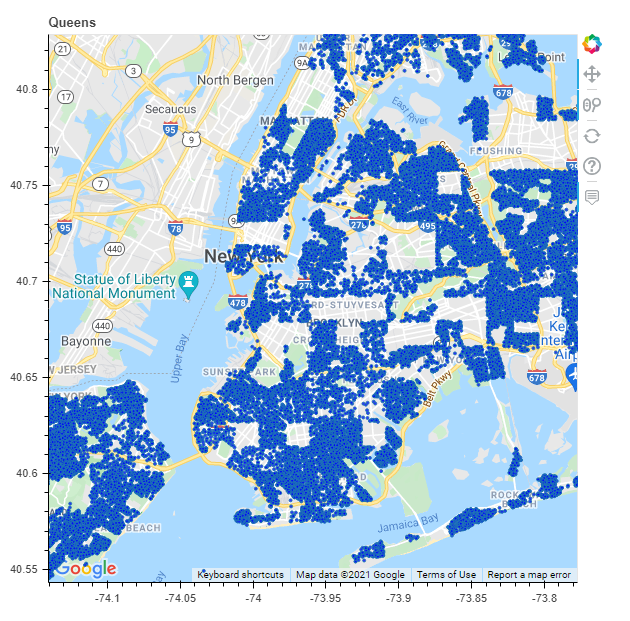
\includegraphics[width=12cm, height=12cm]{NYC_maps_houses.png}
    \end{center}


\section{Exploratory Data Analysis(EDA)}

Exploratory Data Analysis was attempted three times throughout this project, first was done without MICE imputation which is showed in notebook Exploratory-Data-Analysis, a re-do  was done after MICE Imputation showed in notebook inside Redo folder called Data Visualization and EDA and a final was done showed in the notebook analysis-test.\\
\\
There were various findings but the most important was how influential location was compared to other factors. Even with homes with much more luxuries paled in comparison to homes in select areas. You could have a house on Staten Island with 6 bedrooms and 3 bathrooms with over 4000 square and still be more affordable than a home on Manhattan. \\
\subsection{Features}
Features were a key factor in this project and our models needed the right combination to be effective. One of many roadblocks with this data set was working with this feature set not only did many features having missing values, others had wrong entries and ultimately as we will see it was difficult to properly predict. \\
\\
In order find the relations of features on price I looked into a Spearman correlation of all features to other features. A Spearman rank correlation is a non-parametric assessment which measures the level of interconnection between two variables in our case two features. Spearman correlation is done by taking the Pearson correlation coefficient on ranked data and making $\rho$ between $-1$ and $1$ which determines the two variables relationship. As $\rho$ deviates further away from zero leans toward $1$ or $-1$ the stronger the relationship is. If $\rho$ is towards 1 it indicates if one variable increase so does the other. Whereas if $\rho$ is towards -1 then this indicates as one variable increase the other is likely to decrease.\\

Here is a heatmap of Spearman Correlation of our data set
    \begin{center}
        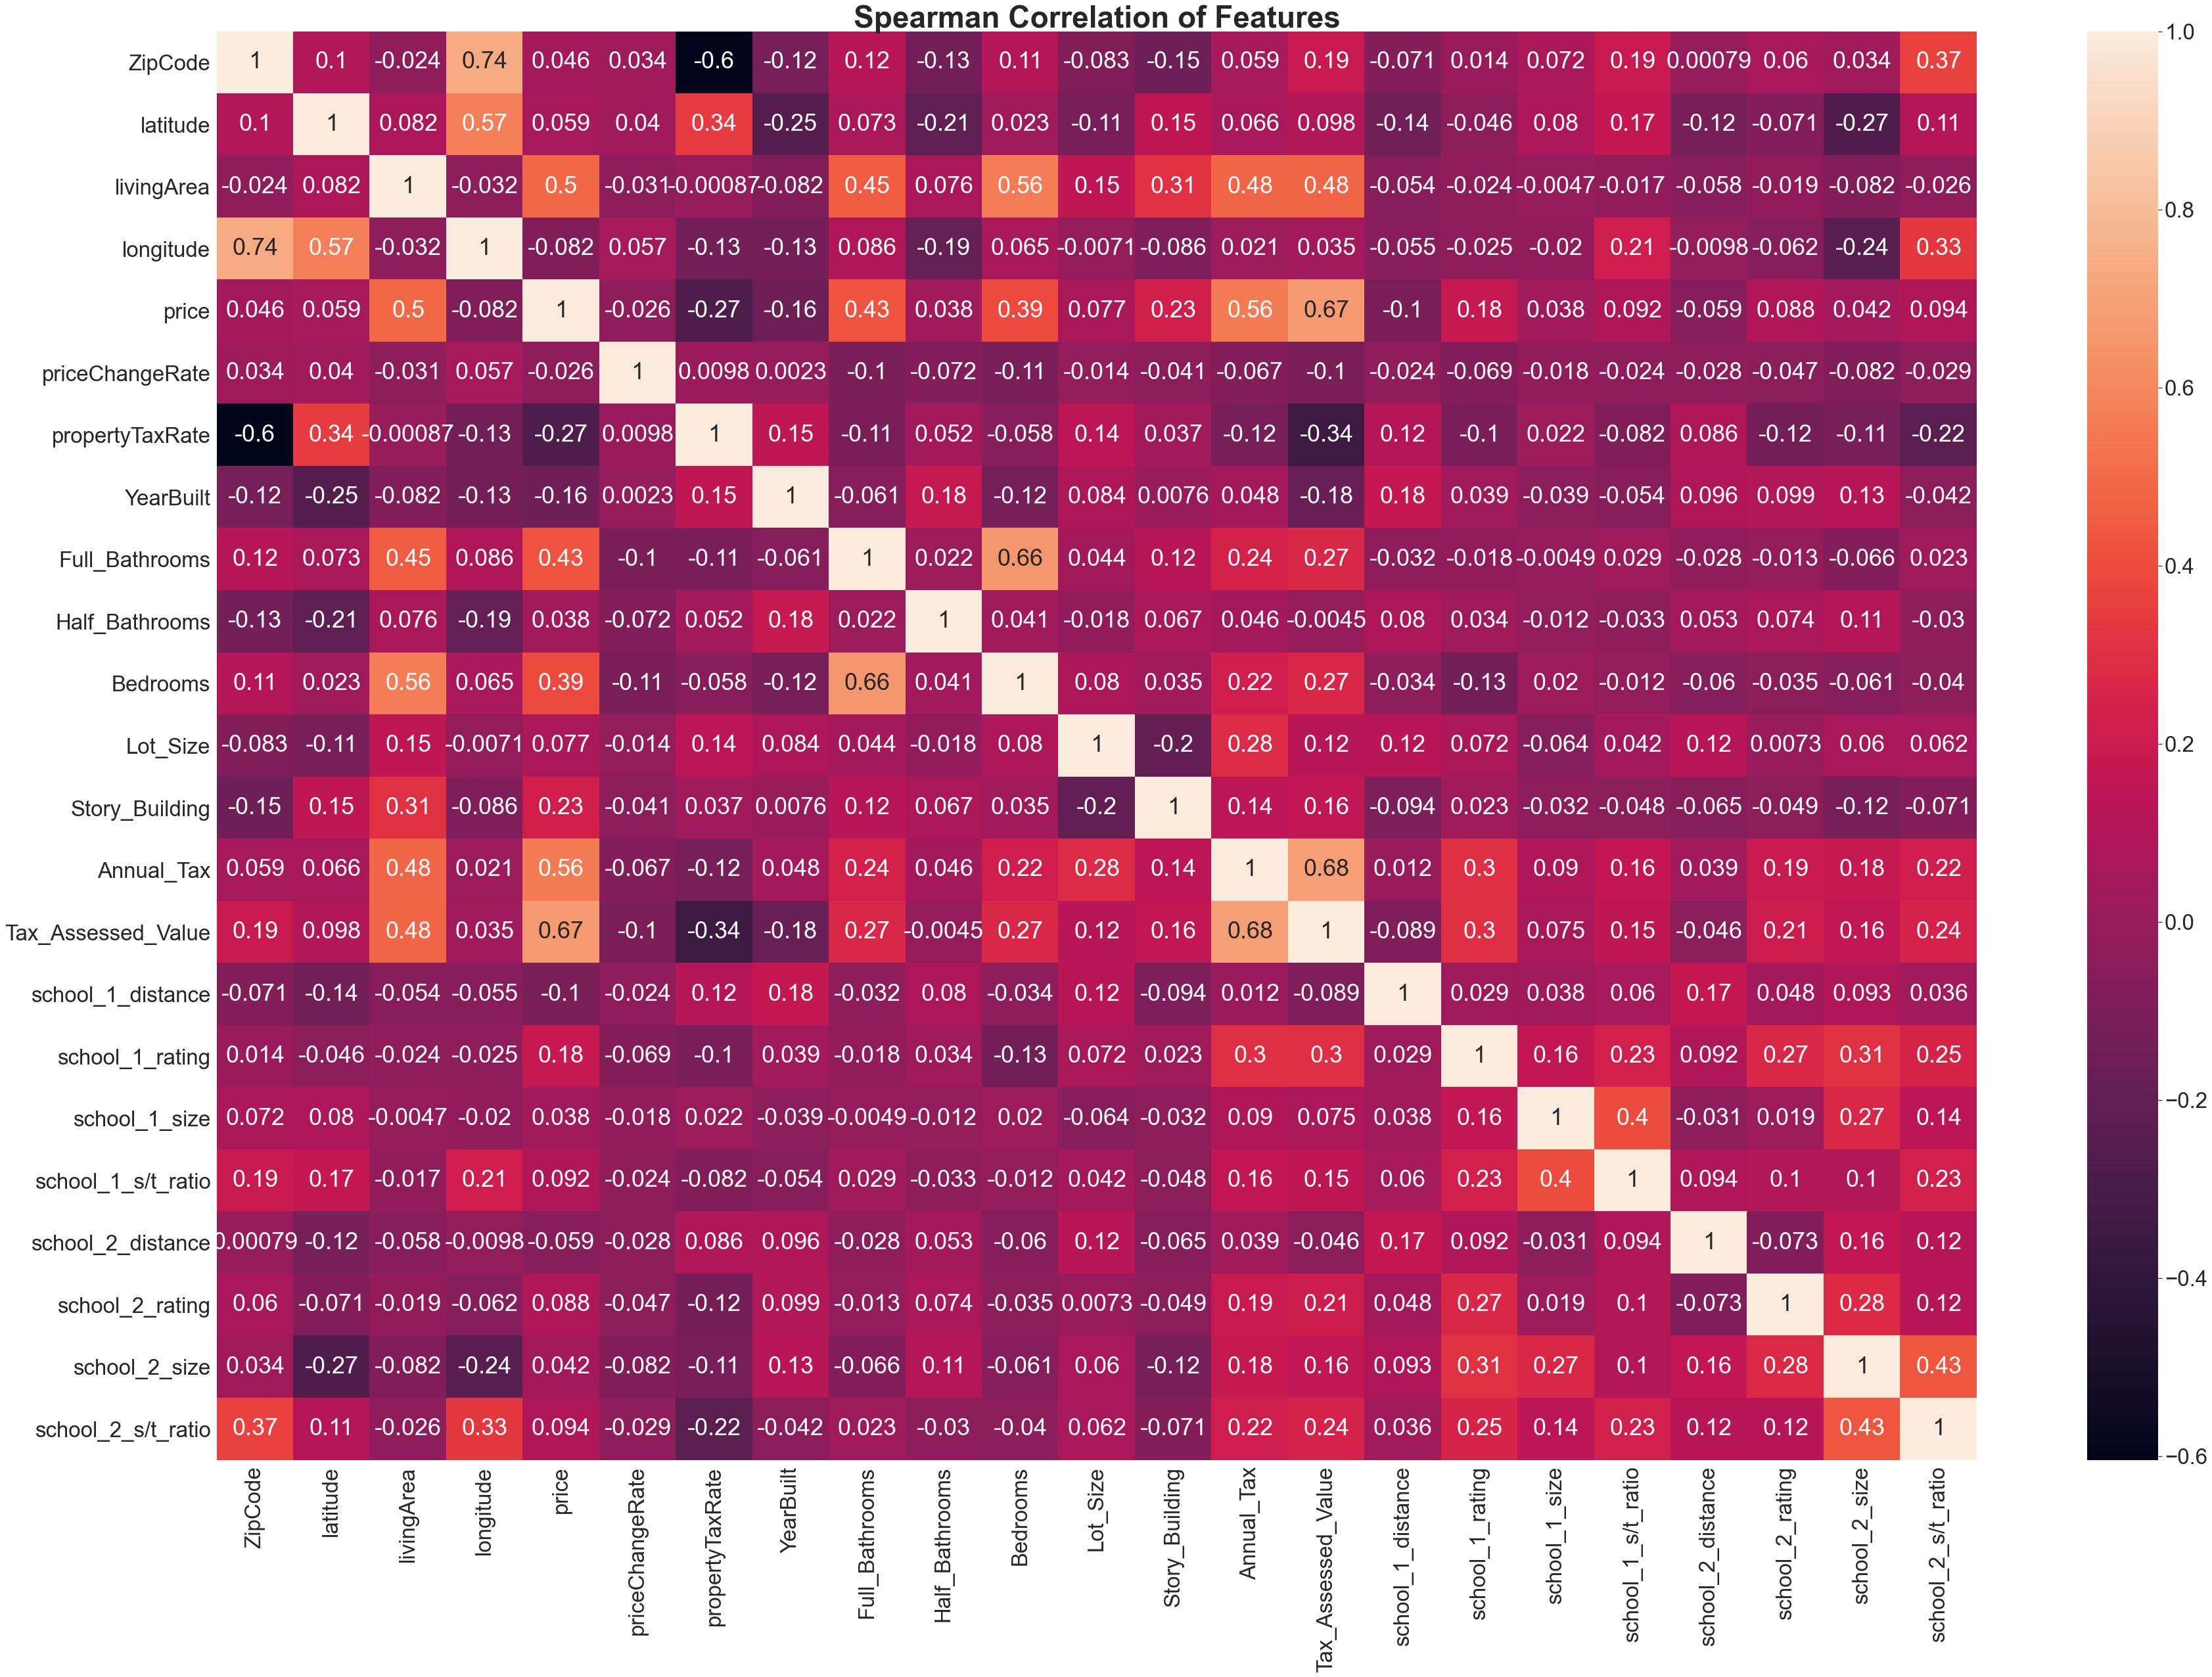
\includegraphics[width=\textwidth,height=\textheight,keepaspectratio]{heatmap.png}
    \end{center}

There is a strong correlation between 'Tax assessed value', 'Annual tax', and 'livingArea' but for the most part it seems there is not a lot of relationship between 'price' and rest of the features so I opted to utilize gradient boosting's and all decision tree neat attribute called feature importance's, this allows us to see which features impacted the most when making decisions. Here is a chart of most important features

\begin{wrapfigure}{r}{0.8\textwidth}
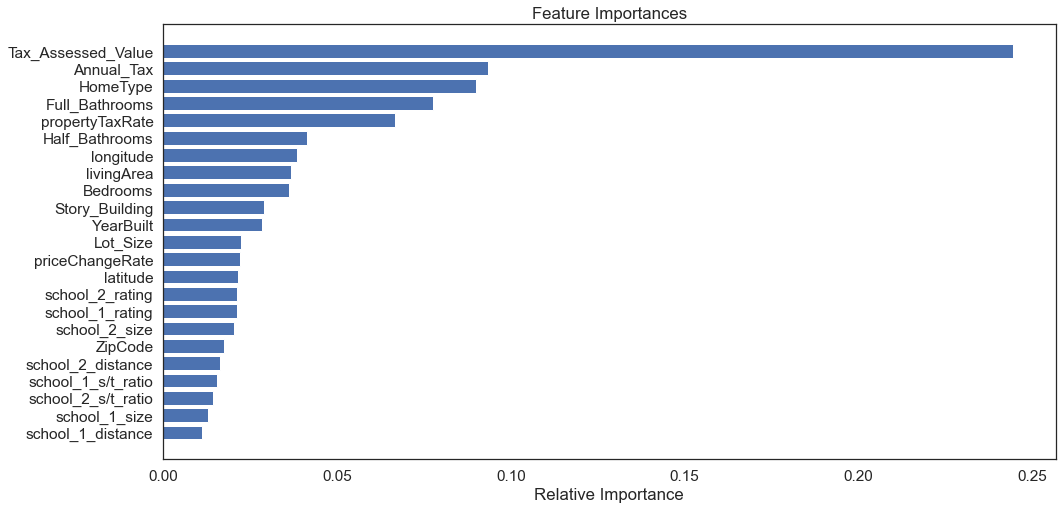
\includegraphics[width=0.85\textwidth, height=0.25\textheight]{features.png}
\label{fig:wrapfig}
\end{wrapfigure}
Like our heatmap Taxes and other highly correlated features have more impact but surprisingly latitude and longitude contributed more than our heatmap might have lead us to believe. This will be further explained once we see how important location really is.
\subsection{Home Distributions}
Looking at distribution of homes in New York City it was interesting to see which price bracket most homes were being sold at.

\begin{figure}[ht]

\begin{subfigure}{.5\textwidth}
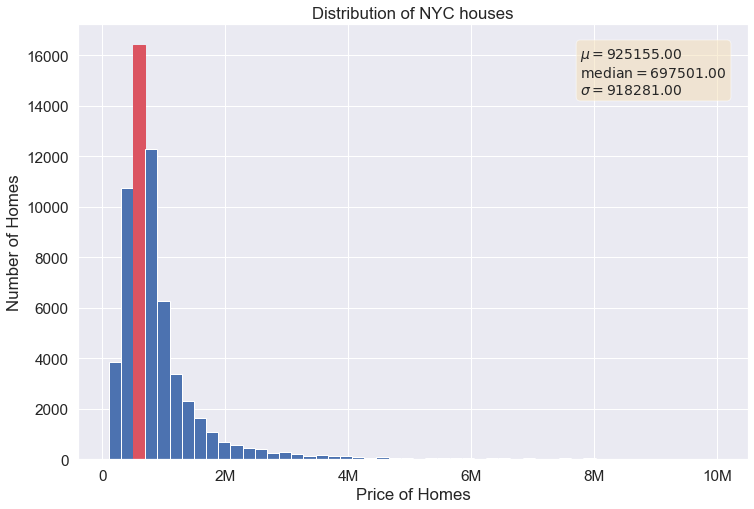
\includegraphics[width=0.95\linewidth]{disthomeprice.png}
\caption{Median Price of New York City nearing $\$700,000$ }
\label{fig:subim1}
\end{subfigure}
\begin{subfigure}{.5\textwidth}
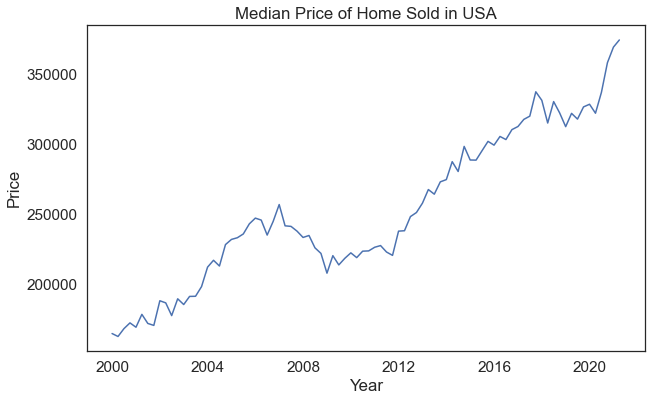
\includegraphics[width=0.95\linewidth]{medprice.png}
\caption{Plot created from data provided from \href{https://fred.stlouisfed.org/series/MSPUS}{Fred}}
\label{fig:subim2}
\end{subfigure}
\newline
\label{fig:image2}
\end{figure}
As the median price of NYC is nears $\$700,000$ it is significantly higher than national median price ($\$400,000$) of homes sold in the USA, showing greater asset appreciation than most markets in USA.
\clearpage





\subsection{Borough Distribution}
While New York City seeks a premium compared to national median house prices, this is further true in New York City's local market as well. We will now look at how each borough of NYC and how homes prices distributed.
\newline
\\

Below is a ridgeline density plot created using \href{https://github.com/leotac/joypy}{joyplot}, density is obtain using Gaussian KDE(Kernel Density Estimate) from scipy library.

\begin{center}
        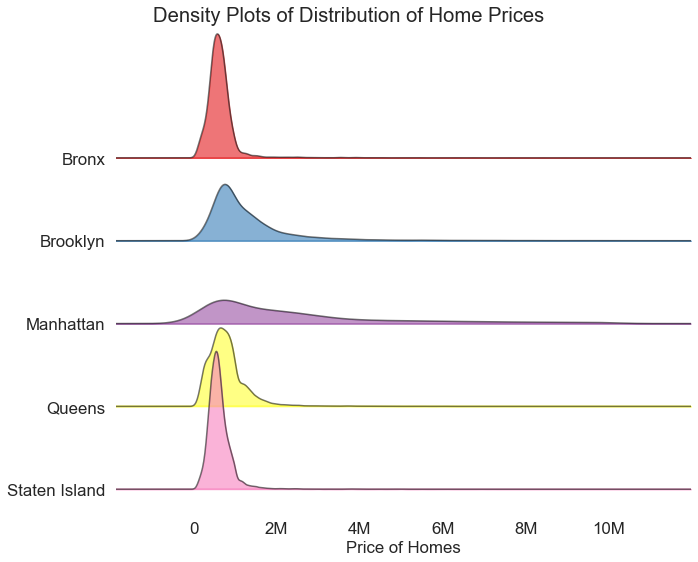
\includegraphics[width=\textwidth,height=\textheight,keepaspectratio]{ridgekdeplot.png}
\end{center}

We can see prices in Manhattan are the most spread, while homes in Bronx, Staten Island are more closely packed. I believe this is due to Manhattan being developed for a much longer period of time thus having more diversification in pricing of homes while the latter have developed much later and are not as sought after. \\
\clearpage

\begin{figure}[ht]

\begin{subfigure}{.5\textwidth}
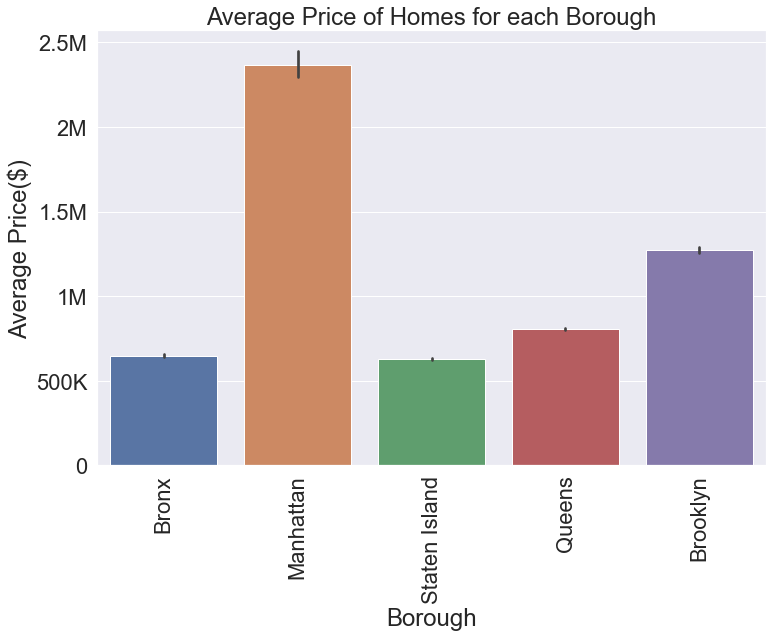
\includegraphics[width=0.95\linewidth]{borough_price.png}
\label{fig:subim3}
\end{subfigure}
\begin{subfigure}{.5\textwidth}
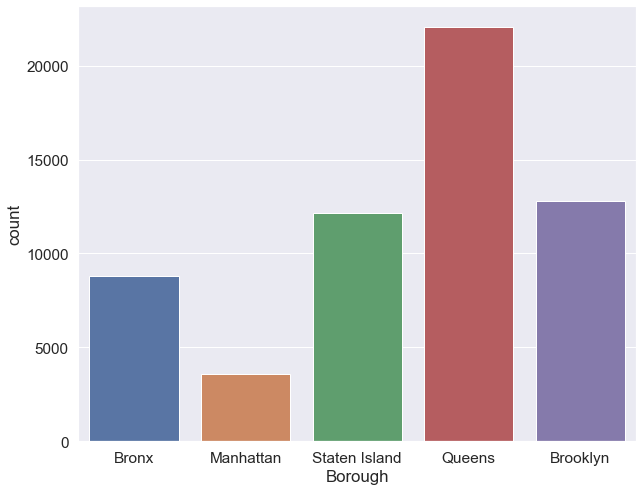
\includegraphics[width=0.95\linewidth]{borough_count.png}
\label{fig:subim4}
\end{subfigure}
\newline
\label{fig:image3}
\end{figure}


Our previous claim seems to have some validity as Manhattan has the least amount of houses for sale but they yield the highest prices, followed by Brooklyn.and Queens, both who have relatively more houses for sale. \\

This indicates how important location really is and explains why we saw longitude and latitude play such a key role, as the clustering of houses based on their coordinates mimicked similar prices thus allowing for better predictions. While in theory this should not have a significant impact as coordinates in this case is not ranked or ordered but we do know typically coordinates which are contained in Manhattan will have higher price value than those outside of it.\\
\\
As we follow the graph below we can see New York City as greatly appreciated, and this even more true for Manhattan who has seen significant gains, note this is only data from 2003-2014 and not recent as this figure is much higher today.
\begin{figure}[ht]

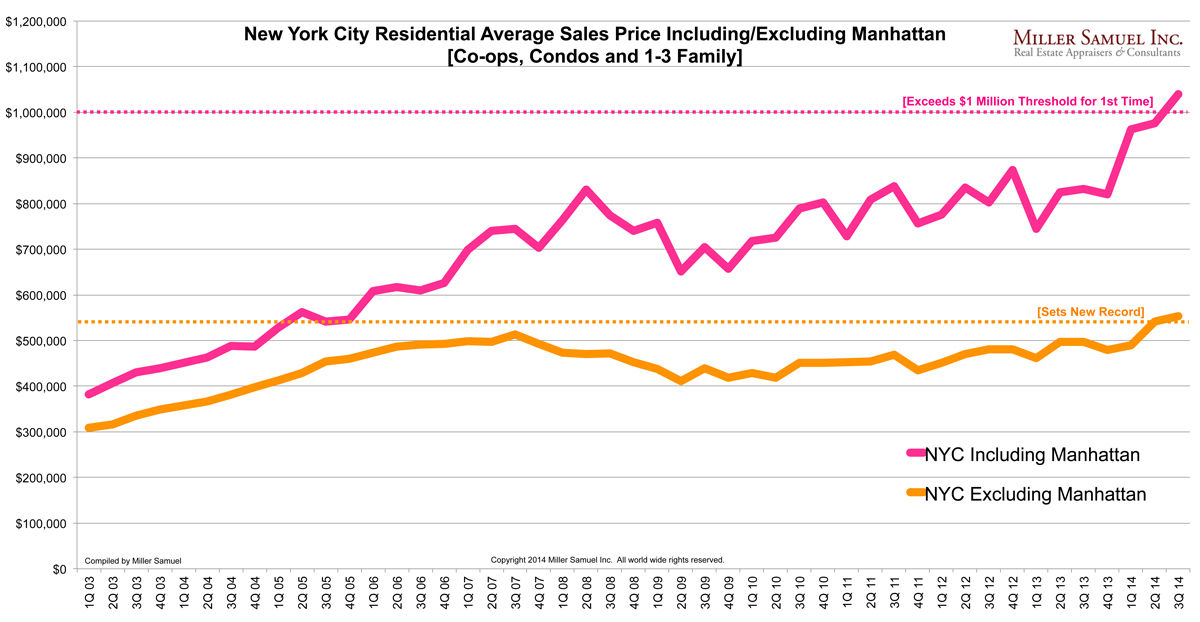
\includegraphics[width=.95\linewidth]{historicalnycprice.jpg}
\caption{Thanks to Miller Samuel Inc. I was able to obtain historical average home prices in New York City from 2003 to 2014. All rights and credit for the following graph goes to this \href{https://www.millersamuel.com/charts/new-york-city-residential-average-sales-price-includingexcluding-manhattan/}{link}}

\end{figure}

\subsection{Years effect on Homes}
Looking into how the year when a house was built and its effects  on the price of the house was surprising. Looking at the chart below of average house price of homes built throughout the years by decades we see during the 1800's and early 1900's have the greatest appreciation, but this is misleading as $70\%$ of all homes were in either Manhattan or Brooklyn. But looking into more recent trends we saw and uptick of average price increases to newer homes and $53\%$ of these homes were in Queens and Staten Island thus not being skewed by high prices of the other boroughs.

\begin{center}
        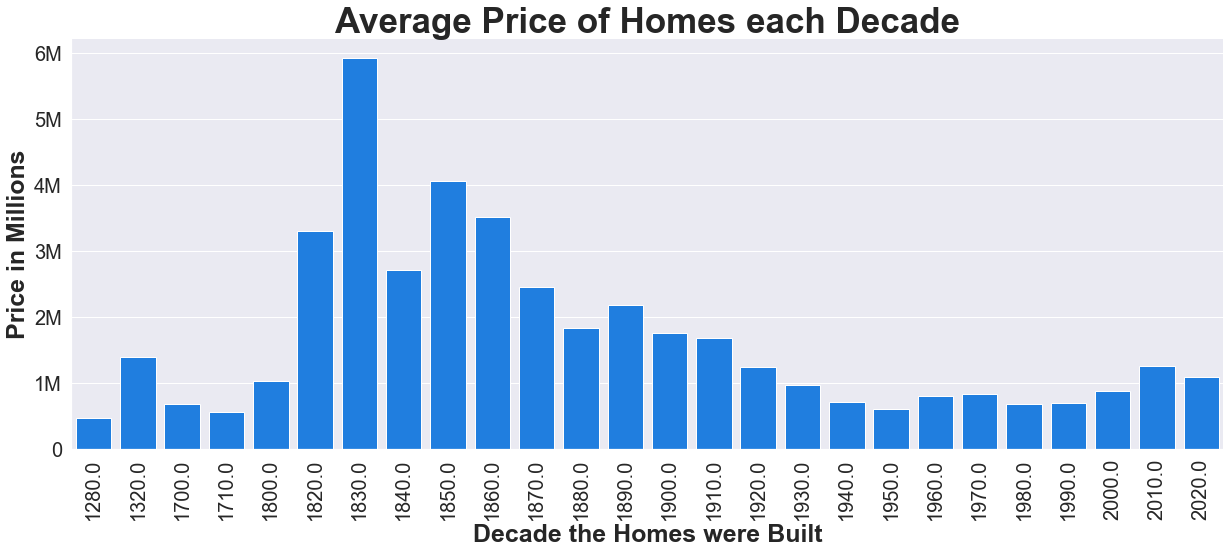
\includegraphics[width=.65\paperwidth, height= .25\paperwidth, keepaspectratio]{houseyearprice.png}
\end{center}

\subsection{Property Type}
I wanted check how a property type and its effect on the house was, but due to the constraints of inaccurate data of this data set it was difficult to pinpoint the specific details of its effects on home price. Nevertheless I  was still able get some insights.
\begin{figure}[H]
\begin{subfigure}{.5\textwidth}
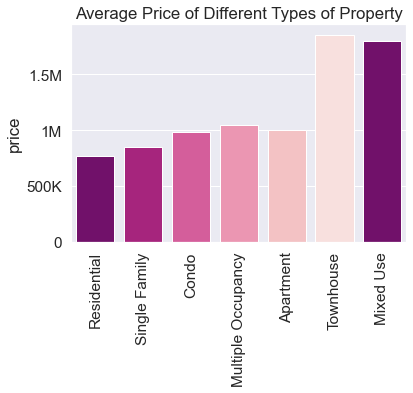
\includegraphics[width=0.95\linewidth]{hometypeprice.png}
\end{subfigure}
\begin{subfigure}{.5\textwidth}
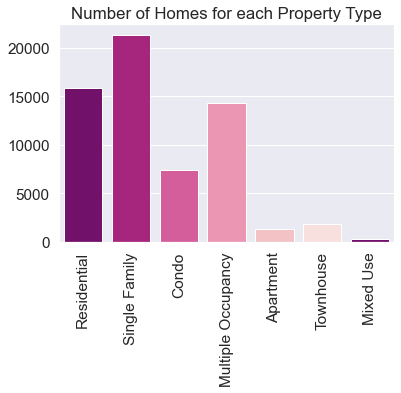
\includegraphics[width=0.95\linewidth]{hometypecount.png}
\end{subfigure}
\end{figure}

\clearpage
I was surprised to see how valuable Townhouses were but looking at the number of Townhouses in the data set we can see this can be easily skewed, same is true for Mixed Use properties.\\
\\
Looking at our findings I believe it is very difficult to pinpoint how much home type influences prices. NYC prices tends to vary heavily on location and so while a Condo might be only $\$200,000$ in Staten Island it can be over $\$2,000,000$ in Manhattan. But it cannot be denied that homes that are meant for condo's and multiple family homes see high valuation. There is always need for housing for families Fortune Capital can always feel secured knowing they built homes for multiple families, if not sold it can always be rented out for passive income.

\section{Model Selection}
\subsection{Metrics of Evaluation}
Selecting the right metric is key in order to evaluate performance, these are the following metrics we will be using to evaluate our models.
\begin{itemize}
  \item R² - R² shows how well terms (data points) fit a curve or line.
  \item MAE - Mean absolute error (On average how far is the prediction from the actual).
  \item MSE - Mean squared error.
  \item RMSE - Root mean squared error. It is the square root of the MSE.
  \item MAPE - Mean Absolute Percentage Error.
\end{itemize}
Ideally you like to see all the metrics improve with each respective model but that is not always the case for that reason we will be using MAE as the main metric
\subsection{Linear Model}
Linear regression model is one of the fundamental models all machine learning course teach, it is machine learning algorithm which relies on supervised learning. Regression models in general dependent value based on its independent variables. It is mostly used for finding out the relationship between variables and predictions. There are different regression model which differ by the kind of interaction dependent and independent variables have.
\\
\begin{wrapfigure}{r}{0.45\textwidth}
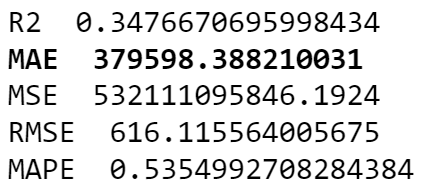
\includegraphics[width=0.3\textwidth, height=0.3\textheight, keepaspectratio]{lm.PNG}
\label{fig:wrapfig2}
\end{wrapfigure}
Here are the results from using LinearRegression from scikit learn package, we can see linear model results are really far from actual price.
\subsection{Nearest Neighbor}


K-Nearest Neighbors is another fundamental but basic classification algorithm used in Machine Learning. It is also based on supervised learning sees usage in application of pattern recognition, data mining and etc. It works by selecting a single data point in the data set and finding the closest 'neighbors' in other words other data points, this is done via a chosen distance formula and given the number of 'K' neighbors that data point is predicted to be the majority of its neighbors.

\begin{center}
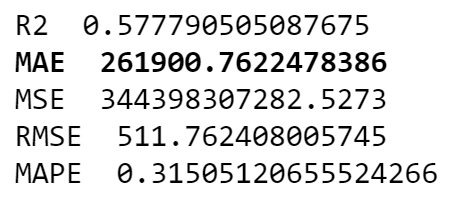
\includegraphics[width=0.3\textwidth, height=0.3\textheight, keepaspectratio]{knn.PNG}
\end{center}

I did further parameter tuning as the number of neighbors selected dictates how well our model does, after some parameter tuning we ended up with an MAE of $249954.9095$, better but not good enough.
\subsection{Random Forest}

Random Forest is an decision which use an ensemble technique being able to perform both regression and classification problems. Utilizing  bootstrapping which randomly samples from the datasets for each tree and performing aggregation, together known as bagging it is able to complete its tasks. It basically combines many decision trees to decide what the final output should rather than only relying on a singular decision tree.

\begin{center}
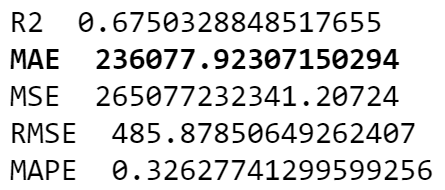
\includegraphics[width=0.3\textwidth, height=0.3\textheight, keepaspectratio]{rf.PNG}
\end{center}

Similarly to tuning Nearest Neighbors, after tuning Random Forest I was able to achieve an MAE of $222413.368$

\subsection{Gradient Boosting}

Our final model Gradient Boosting works by minimizing its past errors, it does this by not tweaking the weighing of training instances, but rather tweaking the predictor such that it is trained by using the residual errors of its predecessors as labels. \\
\\

Jake Hoare does  a beautiful job explaining on how Gradient Boosting works, you can click on this  \href{https://www.geeksforgeeks.org/ml-gradient-boosting/}{link} to see the full webpage

\say{Gradient boosting is a type of machine learning boosting. It relies on the intuition that the best possible next model, when combined with previous models, minimizes the overall prediction error. The key idea is to set the target outcomes for this next model in order to minimize the error. How are the targets calculated? The target outcome for each case in the data depends on how much changing that case's prediction impacts the overall prediction error:
\begin{itemize}
    \item If a small change in the prediction for a case causes a large drop in error, then next target outcome of the case is a high value. Predictions from the new model that are close to its targets will reduce the error.
    \item If a small change in the prediction for a case causes no change in error, then next target outcome of the case is zero. Changing this prediction does not decrease the error.
\end{itemize}
The name gradient boosting arises because target outcomes for each case are set based on the gradient of the error with respect to the prediction. Each new model takes a step in the direction that minimizes prediction error, in the space of possible predictions for each training case.}
\\
\\
From all the models we got the best results from XGBoost's gradient boost and thus we will attempt to try to squeeze better results. We will first make a log-transformation of our target variable of 'price', this will help with outliers or the extremes of very high priced homes which don't contribute to majority of the distribution. Then we will proceed to tune the parameters of XGBoost
\begin{center}
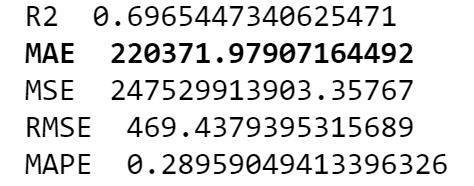
\includegraphics[width=0.3\textwidth, height=0.3\textheight, keepaspectratio]{gb.PNG}
\end{center}

\subsection{Hyper-parameter Tuning}
Hyper parameters are variables in the algorithm we choose that we can tune in our case of XGBoost these values are:
\begin{itemize}
    \item eta - which is the learning rate of our model which is the shrinkage you do at every step you are making, increasing this allows for much faster computation where as decreasing this allows for best optimum result
    \item max depth - controls how complex a model becomes, more depth more likely it is to over-fit where too little leads to simple and underfitting model
    \item min child weight - which is how much weight is placed on each leaf node, the larger it is the more conservative the algorithm will be.
    \item subsample - controls the ratio of training instances, this is the amount of observations to be randomly samples for each tree. Lower values make the algorithm more conservative and prevents overfitting but too small values might lead to under-fitting.
    \item colsample bytree - this is the same as subsample except this is for the columns in other words the features
\end{itemize}

These values control the learning process and determine the values of model parameters that a learning algorithm ends up learning, this is not to be confused for our model's features/variables. The process of tuning might seem simple but the time consumed can be long, its is important to remember even if a better result can be achieved by a lengthy search process but is it worth the time invested. \\
\\
Here are the final results after fine-tuning each of the values listed above.
\begin{center}
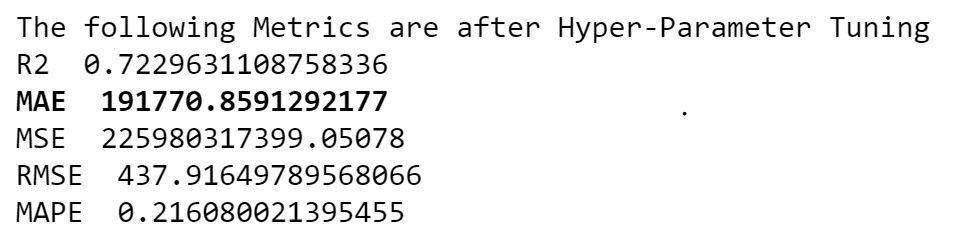
\includegraphics[width=0.7\textwidth, height=0.7\textheight, keepaspectratio]{gbtuned.PNG}
\end{center}
\section{Conclusion}
I found the best results with XGBoost as this led to the most accurate price prediction compared to other models. Coupled with our EDA we have found the most important factor of price of a home is location in New York City. My suggestion to Capital Fortune, if given a choice between the 5 boroughs I would choose Manhattan, then Brooklyn followed by Queens. While it is much more expensive to buy land for construction in Manhattan, we can see that return on investment is also much higher in this location, while Queens has the largest opportunity, as land is far cheaper and cost of construction is relatively equal. I also suggest opting for Single, Multi-Family and Condo's houses as these saw the highest return on investment given our sample size relative to other options.\\
\\
We saw that more expensive houses are older houses but upon a closer look this is because these are homes build in the 1800's and early 1900's in Manhattan and Brooklyn, leading to location being the main driving factor of the price, and many of these houses were remodeled even though their listed built year is older. But notice after the 1950's the average price of houses increases as more recent it is. This puts our clients houses at a premium compared to an older or remodeled old home.\\
\\
On average we can expect homes build in Manhattan to run between 1 to 3 million more compared to other boroughs with an average price of 3 million for a newly build home. Next would be Brooklyn with an average price of 1.2 million for a newly build home and then Queens with 800K. Bronx and Staten Island might not be as lucrative as its neighbors, but they can be much to be desired as a newly build home on Bronx can be around 600K and for Staten Island 500K. \\
\\
Capital Fortune is also poised to make higher returns on their homes as their homes will be brand new construction. With newer homes one can expect an average of $\$50,000-150,000$ premium versus a old or remodeled home.

\section{Personal Takeaways and Further Study}

This was a tedious and interesting project to work on, working with such dirty raw data really gave me and appreciation for data collection and integrity. It really changed my perspective and learning experience on how to properly clean and wrangle data. I would like to see how different results would have been in different markets as NYC is a very sought after and the gap between Manhattan compared to Bronx or Staten Island is staggering.
\\
\\
I believe there is more data we can compile for better predictions for instances the construction costs of homes, or prices of goods and services in the proximity of the house. I would love to continue this and look into the whole United States housing market and how different cities, or states compare and how different features impact the overall market compared to local markets.


\end{titlepage}
\end{document}
